
\documentclass[12pt,a4paper, oneside]{extreport}

%%%%%%%%%% Математика %%%%%%%%%%
\usepackage{amsmath,amsfonts,amssymb,amsthm,mathtools}
% Показывать номера только у тех формул, на которые есть \eqref{} в тексте.
%\mathtoolsset{showonlyrefs=true}
%\usepackage{leqno} % Нумерация формул слева
%\usepackage{tipa} %Для формулки из логитов


\usepackage{hyphenat}

%%%%%%%%%% Шрифты %%%%%%%%
\usepackage[english, russian]{babel} % выбор языка для документа
\usepackage[utf8]{inputenc} % задание utf8 кодировки исходного tex файла
\usepackage[X2,T2A]{fontenc}        % кодировка

\usepackage{fontspec}         % пакет для подгрузки шрифтов
\setmainfont{Times New Roman}       % задаёт основной шрифт документа

\usepackage{unicode-math}      % пакет для установки математического шрифта
%\setmathfont{Asana-Math.otf}    % шрифт для математики

% Конкретный символ из конкретного шрифта
% \setmathfont[range=\int]{Neo Euler}


%%%%%%%%%% Работа с картинками %%%%%%%%%
\usepackage{graphicx}                  % Для вставки рисунков
\usepackage{graphics}
\graphicspath{{images/}{pictures/}}    % можно указать папки с картинками
\usepackage{wrapfig}                   % Обтекание рисунков и таблиц текстом


%%%%%%%%%% Работа с таблицами %%%%%%%%%%
\usepackage{tabularx}            % новые типы колонок
\usepackage{tabulary}            % и ещё новые типы колонок
\usepackage{array,delarray}      % Дополнительная работа с таблицами
\usepackage{longtable}           % Длинные таблицы
\usepackage{multirow}            % Слияние строк в таблице
\usepackage{float}               % возможность позиционировать объекты в нужном месте

\usepackage{booktabs}            % таблицы как в книгах

% Заповеди из документации к booktabs:
% 1. Будь проще! Глазам должно быть комфортно
% 2. Не используйте вертикальные линни
% 3. Не используйте двойные линии. Как правило, достаточно трёх горизонтальных линий
% 4. Единицы измерения - в шапку таблицы
% 5. Не сокращайте .1 вместо 0.1
% 6. Повторяющееся значение повторяйте, а не говорите "то же"
% 7. Есть сомнения? Выравнивай по левому краю!

%  вычисляемые колонки по tabularx
\newcolumntype{C}{>{\centering\arraybackslash}X}
\newcolumntype{L}{>{\raggedright\arraybackslash}X}
\newcolumntype{Y}{>{\arraybackslash}X}
\newcolumntype{Z}{>{\centering\arraybackslash}X}


%%%%%%%%%% Графика и рисование %%%%%%%%%%
\usepackage{tikz, pgfplots}      % язык для рисования графики из latex'a

%%%%%%%%%% Гиперссылки %%%%%%%%%%
\usepackage{xcolor}              % разные цвета

\usepackage{hyperref}
\hypersetup{
	unicode=true,           % позволяет использовать юникодные символы
	colorlinks=true,       	% true - цветные ссылки, false - ссылки в рамках
	urlcolor =blue,         % цвет ссылки на url
	linkcolor=black,        % внутренние ссылки
	citecolor=black,        % на библиографию
	breaklinks              % если ссылка не умещается в одну строку, разбивать ли ее на две части?
}


%%%%%%%%%% Другие приятные пакеты %%%%%%%%%
\usepackage{multicol}       % несколько колонок
\usepackage{verbatim}       % для многострочных комментариев
\usepackage{cmap} % для кодировки шрифтов в pdf

\usepackage{enumitem} % дополнительные плюшки для списков
%  например \begin{enumerate}[resume] позволяет продолжить нумерацию в новом списке

\usepackage{todonotes} % для вставки в документ заметок о том, что  осталось сделать
% \todo{Здесь надо коэффициенты исправить}
% \missingfigure{Здесь будет Последний день Помпеи}
% \listoftodos --- печатает все поставленные \todo'шки



%%%%%%%%%%%%%% ГОСТОВСКИЕ ПРИБАМБАСЫ %%%%%%%%%%%%%%%

%%% размер листа бумаги
\usepackage[paper=a4paper,top=15mm, bottom=15mm,left=35mm,right=10mm,includehead]{geometry}


\usepackage{setspace}
\setstretch{1.5}     % Межстрочный интервал
\setlength{\parindent}{1.25cm} % Красная строка.


%\flushbottom       % Эта команда заставляет LaTeX чуть растягивать строки, чтобы получить идеально прямоугольную страницу
\righthyphenmin=2  % Разрешение переноса двух и более символов
\widowpenalty=10000  % Наказание за вдовствующую строку (одна строка абзаца на этой странице, остальное --- на следующей)
\clubpenalty=10000  % Наказание за сиротствующую строку (омерзительно висящая одинокая строка в начале страницы)
\tolerance=1000     % Ещё какое-то наказание.


% Нумерация страниц сверху по центру
\usepackage{fancyhdr}
\pagestyle{fancy}
%\fancyhead{ } % clear all fields
%\fancyfoot{ } % clear all fields
\fancyhf{}
\fancyhead[R]{Касьянова Ксения, Шуляк Елена (СМАР19)}
\fancyfoot[C]{\thepage}
% Чтобы не прорисовывалась черта!
\renewcommand{\headrulewidth}{0pt}


% Нумерация страниц с надписью "Глава"
\usepackage{etoolbox}
\patchcmd{\chapter}{\thispagestyle{plain}}{\thispagestyle{fancy}}{}{}


%%% Заголовки
\usepackage[indentfirst]{titlesec}{\raggedleft}
% Заголовки по левому краю
% опция identfirst устанавливает отступ в первом абзаце



% В Linux этот пакет сделан косячно. Исправляет это следующий непонятный кусок кода.
\makeatletter
\patchcmd{\ttlh@hang}{\parindent\z@}{\parindent\z@\leavevmode}{}{}
\patchcmd{\ttlh@hang}{\noindent}{}{}{}
\makeatother


% Редактирования Глав и названий
\titleformat{\chapter}
{\normalfont\large\bfseries}
{\thechapter }{0.5 em}{}

% Редактирование ненумеруемых глав chapter* (Введение и тп)
\titleformat{name=\chapter,numberless}
{\centering\normalfont\bfseries\large}{}{0.25em}{\normalfont}

% Убирает чеканутые отступы вверху страницы
\titlespacing{\chapter}{0pt}{-\baselineskip}{\baselineskip}

% Более низкие уровни
\titleformat{\section}{\bfseries}{\thesection}{0.5 em}{}
\titleformat{\subsection}{\bfseries}{\thesubsection}{0.5 em}{}

\titlespacing*{\section}{0 pt}{\baselineskip}{\baselineskip}
\titlespacing*{\subsection}{0 pt}{\baselineskip}{\baselineskip}


% Содержание. Команды ниже изменяют отступы и рисуют точечки!
\usepackage{titletoc}

\titlecontents{chapter}
[1em] %
{\normalsize}
{\contentslabel{1 em}}
{\hspace{-1 em}}
{\normalsize\titlerule*[10pt]{.}\contentspage}

\titlecontents{section}
[3 em] %
{\normalsize}
{\contentslabel{1.75 em}}
{\hspace{-1.75 em}}
{\normalsize\titlerule*[10pt]{.}\contentspage}

\titlecontents{subsection}
[6 em] %
{\normalsize}
{\contentslabel{3 em}}
{\hspace{-3 em}}
{\normalsize\titlerule*[10pt]{.}\contentspage}


% Правильные подписи под таблицей и рисунком
% Документация к пакету на русском языке!
\usepackage[tableposition=top, singlelinecheck=false]{caption}
\usepackage{subcaption}


\DeclareCaptionStyle{base}%
[justification=centering,indention=0pt]{}
\DeclareCaptionLabelFormat{gostfigure}{Рисунок #2}
\DeclareCaptionLabelFormat{gosttable}{Таблица #2}

\DeclareCaptionLabelSeparator{gost}{~---~}
\captionsetup{labelsep=gost}

\DeclareCaptionStyle{fig01}%
[margin=5mm,justification=centering]%
{margin={3em,3em}}
\captionsetup*[figure]{style=fig01,labelsep=gost,labelformat=gostfigure,format=hang}

\DeclareCaptionStyle{tab01}%
[margin=5mm,justification=centering]%
{margin={3em,3em}}
\captionsetup*[table]{style=tab01,labelsep=gost,labelformat=gosttable,format=hang}


% межстрочный отступ в таблице
\renewcommand{\arraystretch}{1.2}



% многостраничные таблицы под РОССИЙСКИЙ СТАНДАРТ
% ВНИМАНИЕ! Обязательно за CAPTION !
\usepackage{fr-longtable}



%Более гибкие спсики
\usepackage{enumitem}
% сообщаем окружению о том, что существует такая штук как нумерация русскими буквами.
\makeatletter
\AddEnumerateCounter{\asbuk}{\russian@alph}{щ}
\makeatother


%%% ГОСТОВСКИЕ СПИСКИ

% Первый тип списков. Большая буква.
\newlist{Enumerate}{enumerate}{1}

\setlist[Enumerate,1]{labelsep=0.5em,leftmargin=1.25em,labelwidth=1.25em,
	parsep=0em,itemsep=0em,topsep=0ex, before={\parskip=-1em},label=\arabic{Enumeratei}.}


% Второй тип списков. Маленькая буква.
\setlist[enumerate]{label=\arabic{enumi}),parsep=0em,itemsep=0em,topsep=0.75ex, before={\parskip=-1em}}


% Третий тип списков. Два уровня.
\newlist{twoenumerate}{enumerate}{2}
\setlist[twoenumerate,1]{itemsep=0mm,parsep=0em,topsep=0.75ex,, before={\parskip=-1em},label=\asbuk{twoenumeratei})}
\setlist[twoenumerate,2]{leftmargin=1.3em,itemsep=0mm,parsep=0em,topsep=0ex, before={\parskip=-1em},label=\arabic{twoenumerateii})}


% Четвёртый тип списков. Список с тире.
\setlist[itemize]{label=--,parsep=0em,itemsep=0em,topsep=0ex, before={\parskip=-1em},after={\parskip=-1em}}


%%% WARNING WARNING WARNIN!
%%% Если в списке предложения, то должна по госту стоять точка после цифры => команда Enumerate! Если идет перечень маленьких фактов, не обособляемых предложений то после цифры идет скобка ")" => команда enumerate! Если перечень при этом ещё и двууровневый, то twoenumerate.




%%%%%%%%%% Список литературы %%%%%%%%%%

%\usepackage[%
%backend=biber, %подключение пакета biber (тоже нужен)
%bibstyle=gost-numeric, %подключение одного из четырех главных стилей biblatex-gost
%sorting=ntvy, %тип сортировки в библиографии
%]{biblatex}

\usepackage[backend=biber,style=gost-numeric, maxbibnames=9,maxcitenames=2,uniquelist=false, babel=other]{biblatex}



% Справка по 4 главным стилям для ленивых:
% gost-inline  ссылки внутри теста в круглых скобках
% gost-footnote подстрочные ссылки
% gost-numeric затекстовые ссылки
% gost-authoryear тоже затекстовые ссылки, но немного другие

% Подробнее смотри страницу 4 документации. Она на русском.

% Ещё немного настроек
\DeclareFieldFormat{postnote}{#1} %убирает с. и p.
\renewcommand*{\mkgostheading}[1]{#1} % только лишь убираем курсив с авторов






\begin{document} % Начала документа



\chapter{ДЗ-02}


\section{Задача 1.}


\subsection{Построение модели оценки за экзамен.}

Во-первых, по имеющимся данным мы сможем оценить только их влияние на оценку за второй экзамен, так как данные агрегированы за весь семестр.

Во-вторых имеет смысл вместо суммы баллов за домашние задания использовать средний балл, так как он точнее отражает качество выполнения домашнего задания:

\begin{equation}\label{key}
MHW_i = \dfrac{SHW_i}{NHW_i}
\end{equation}

Для определения влияния различных факторов на оценки построим модель, включающую в себя все объективные характеристики, а также дамми на пол: 

\begin{figure}[h!]
	\centering
	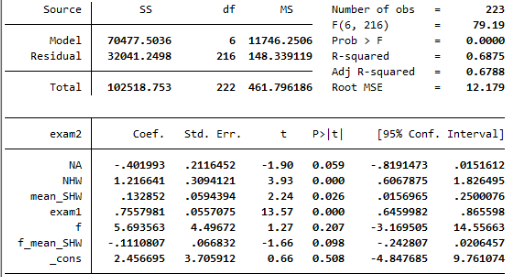
\includegraphics[width=0.7\linewidth]{screenshot001}
	\label{fig:screenshot001}
\end{figure}

Сразу заметим, что коэффициент при количестве посещенных семинаров значим и меньше 0. Можно подумать, что если не сходить 10 семинаров при прочих равных можно получить оценку на 4 балла выше, что очевидно не так. Причиной этому явлется тот факт, что в регрессии есть пропущенные переменные, отвечающая за знания эконометрики на момент начала курса и  ''талант'', который позволяет студентов быстро готовиться за ночь до экзамена. 

Можно предположить, что переменная $Expect$ частично отражает эти факторы, так как высокую оценку будут ожидать только те, кто более-менее уверен в своих знаниях: 

\begin{figure}[h!]
	\centering
	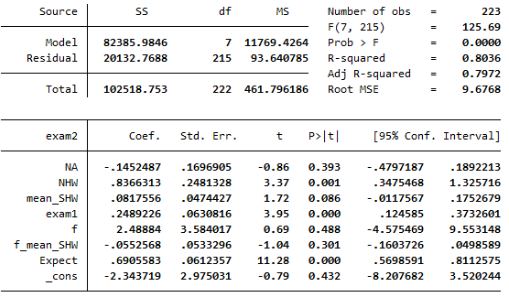
\includegraphics[width=0.7\linewidth]{screenshot002}
%	\caption{}
	\label{fig:screenshot002}
\end{figure}



Действительно, добавив $Expect$ в регрессию видим, что эта переменная значима, а количество посещенных семинаров $NA$ -- нет, также теперь нет различия во влиянии среднего балла на оценки в зависимости от пола. Все это позволяет сделать вывод,  что из-за пропущенной переменной оценки были несостоятельными, а $Expect$ из регрессии убирать не стоит.

Проверим с помощью F-теста гипотезу об одновременном равенстве коэффициентов при $NA$, $f$, $f*MHW$:

\begin{figure}[h!]
	\centering
	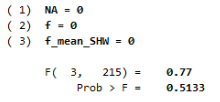
\includegraphics{screenshot003}
%	\caption{}
	\label{fig:screenshot003}
\end{figure}

Согласно результатам теста далее будем использовать короткую модель:

\begin{figure}[h!]
	\centering
	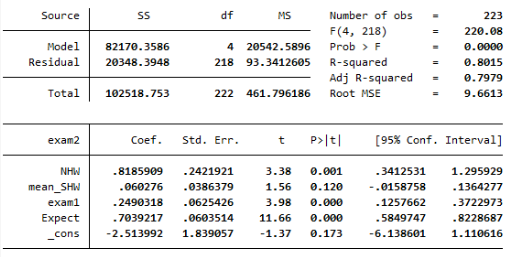
\includegraphics[width=0.7\linewidth]{screenshot004}
%	\caption{}
	\label{fig:screenshot004}
\end{figure}

\newpage

Визуально и согласно критерию Шапиро-Уилка нет оснований предполагать что остатки не распределены нормально:

\begin{figure}[h!]
	\centering
	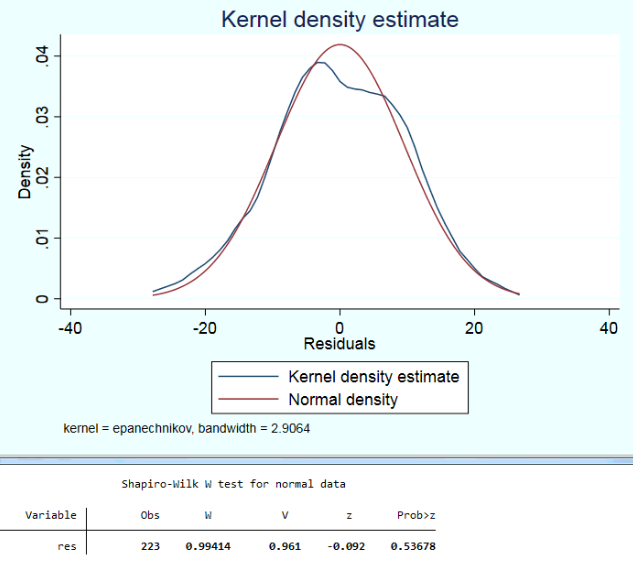
\includegraphics[width=0.7\linewidth]{screenshot005}
%	\caption{}
	\label{fig:screenshot005}
\end{figure}


Также согласно тесту Бройша-Пагана гипотеза о гомоскедастичности ошибок не отвергается:

\begin{figure}[h!]
	\centering
	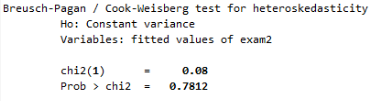
\includegraphics{screenshot006}
%	\caption{}
	\label{fig:screenshot006}
\end{figure}

У модели также достаточно высокий коэффициент детерминации. Поэтому можем считать модель ''хорошей''. Согласно полученным оценкам можно сделать вывод, что количество сданных домашних заданий, оценка за 1-ый экзамен и ожидания положительно влияют на оценку за 2-ой экзамен (менее чем на 1\% уровне значимости), что согласуется с логикой. 


\newpage

\subsection{Построение модели  ожидаемой оценки за экзамен.}


Далее определим, какие факторы могут влиять на ожидания. Построим модель, включающую в себя все объективные характеристики:

\begin{figure}[h!]
	\centering
	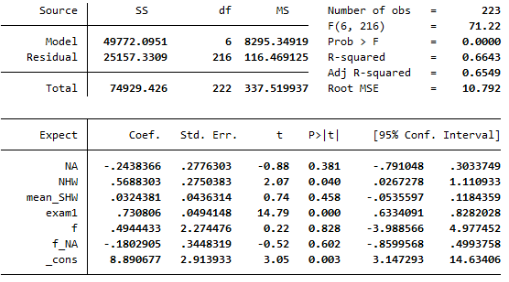
\includegraphics[width=0.7\linewidth]{screenshot007}
%	\caption{}
	\label{fig:screenshot007}
\end{figure}




Вероятно, в этой модели есть пропущенные переменные такого же рода, однако их влияние должно быть не так критично, как в предыдущем случае, поскольку  ожидания зависят не только от способностей экзаменуемого, но также и от  особенностей экзамена.


Согласно тесту Бройша-Пагана  ошибки в этой модели гетероскедастичны: 

\begin{figure}[h!]
	\centering
	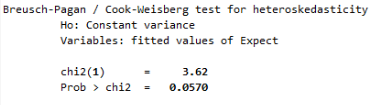
\includegraphics{screenshot008}
%	\caption{}
	\label{fig:screenshot008}
\end{figure}

\newpage

Визуально можно определить, что причиной гетероскедастичности является переменная $NHW$, поскольку большинство студентов сдавали домашние задания, из-за чего у больших значений $NHW$ больше разброс:

\begin{figure}
	\centering
	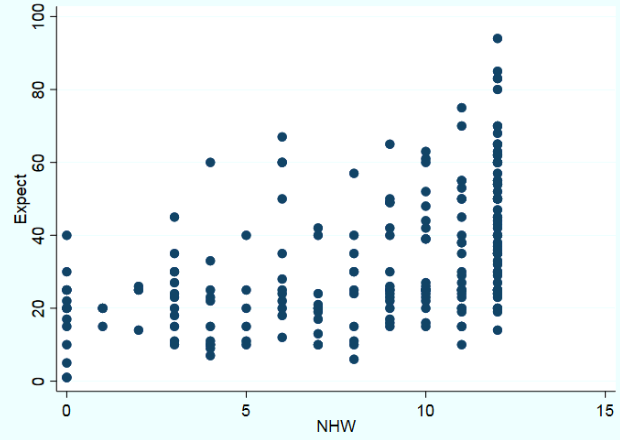
\includegraphics[width=0.7\linewidth]{screenshot009}
%	\caption{}
	\label{fig:screenshot009}
\end{figure}

Поэтому имеет смысл взвесить регрессию по $HNW$, а также использовать робастные оценки ковариационной матрицы HC3:

\begin{figure}[h!]
	\centering
	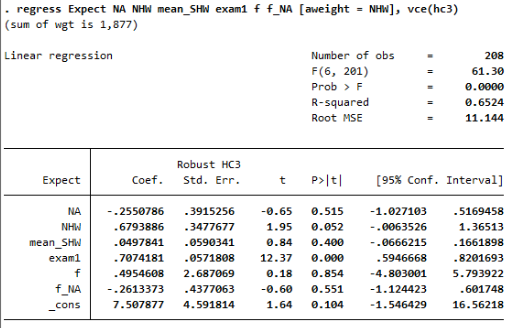
\includegraphics[width=0.7\linewidth]{screenshot010}
%	\caption{}
	\label{fig:screenshot010}
\end{figure}


Cогласно тесту Бройша-Пагана проблема гетероскедастичности частично решена:

\begin{figure}[h!]
	\centering
	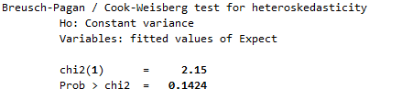
\includegraphics{screenshot011}
%	\caption{}
	\label{fig:screenshot011}
\end{figure}

Поэтому теперь можно пользоваться t-статистиками для определения значимости коэффициентов регрессии. 

Проверим с помощью F-теста одновременное равенство нулю коэффициентов при $MHW$, $f$, $f*NA$:

\begin{figure}[h!]
	\centering
	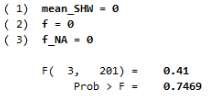
\includegraphics{screenshot012}
%	\caption{}
	\label{fig:screenshot012}
\end{figure}

По результатам F-теста оценим ограниченную регрессию:

\begin{figure}[h!]
	\centering
	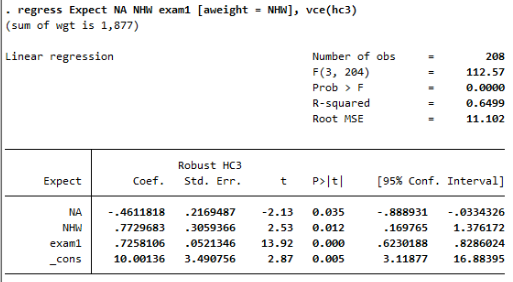
\includegraphics[width=0.7\linewidth]{screenshot013}
%	\caption{}
	\label{fig:screenshot013}
\end{figure}


\begin{figure}[h!]
	\centering
	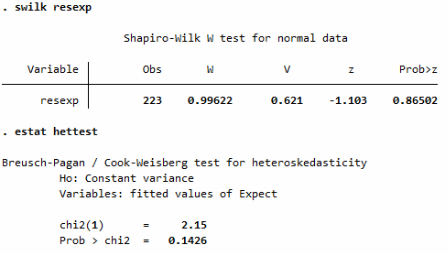
\includegraphics[width=0.7\linewidth]{screenshot014}
%	\caption{}
	\label{fig:screenshot014}
\end{figure}


Ошибки нормальны и гомоскедастичны. $R^2$ достаточно большой. Поэтому по данной модели имеем положительну связь между числом выполненных заданий и оценкой за 2-ой экзамен (на 5\% уровне значимости), положительну связь между оценкой за 1-ый экзамен и оценкой за 2-ой экзамен (менее, чем на 1\% уровне значимости), отрицательную свзяь между числом посещенных семинаров и оценкой за 2-ой экзамен (на 5\% уровне значимости). Последнее, вероятно, можно объяснить тем, что из-за пропущенной переменной отвечающей за начальные эконометрические навыки студента, мы видим это влияние через переменную $NA$, которая на самом деле отражает не прямую связь между прогулами семинаров и ростом оценки за экзамен, а косвенную через тот факт, что те кто не ходят на семинары предполагают, что знают эконометрику, а соответственно и выше оценивают свои ожидания за экзамен.    
 

\subsection{Построение модели  точности прогноза.}


Чтобы определить, насколько точно предсказывают оценку за экзамен студенты, построим регрессию оценок за экзамен на ожидания студентов:

\begin{figure}[h!]
	\centering
	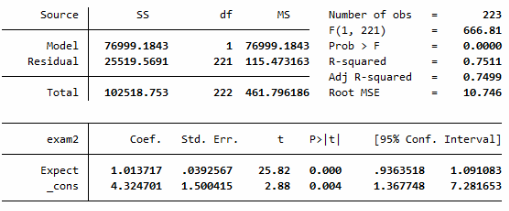
\includegraphics[width=0.7\linewidth]{screenshot015}
%	\caption{}
	\label{fig:screenshot015}
\end{figure}


Можно заметить, что коэффициент при $Expect$ примерно равен 1 (причем $t_{\{H_0:\beta = 1\}} = \frac{\hat{\beta} - 1}{se_{\beta}}$ = 25.82 - 1/0.0393 = 0.3466), а по метрике RMSE можно увидеть, что студенты в среднем ошибаются в своих расчетах на 10 баллов. То есть относительно точно прогнозируют свои оценки.

Для того, чтобы определить, какие факторы влияют на точность прогноза введем переменную    ошибка прогноза в долях $PFE_i = \dfrac{exam_i - \widehat{exam}_i}{exam_i}$:  

\begin{figure}[h!]
	\centering
	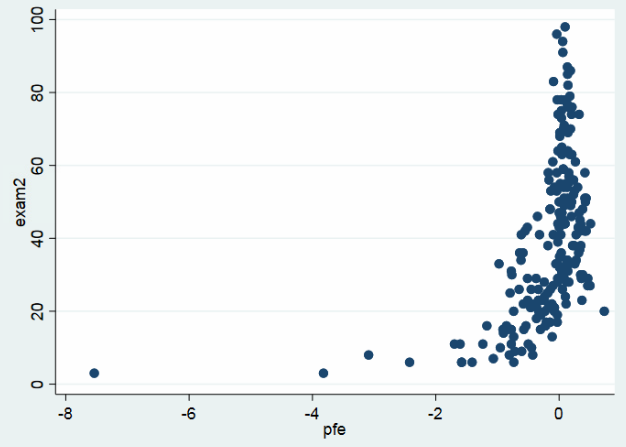
\includegraphics[width=0.6\linewidth]{screenshot016}
%	\caption{}
	\label{fig:screenshot016}
\end{figure}

\newpage

Так как для ответа на поставленный вопрос не важно, кто завысил, а кто занизил свои ожидания, возьмем этот показатель по модулю, а также возьмем логарифм от этой переменной (из-за взятия логарифма на 2 наблюдения меньше):


\begin{figure}[h!]
	\centering
	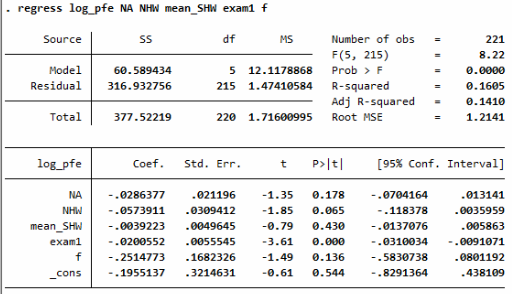
\includegraphics[width=0.7\linewidth]{screenshot017}
%	\caption{}
	\label{fig:screenshot017}
\end{figure}


\begin{figure}[h!]
	\centering
	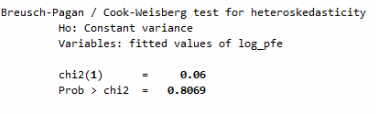
\includegraphics{screenshot018}
%	\caption{}
	\label{fig:screenshot018}
\end{figure}


Ошибки гомоскедастичны (но на всякий случай будем использовать робастные оценки), поэтому воспользуемся F-тестом, чтобы проверить значимость коэффициентов при $NA$, $MHW$, $f$

\begin{figure}[h!]
	\centering
	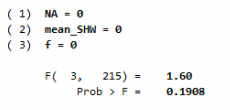
\includegraphics{screenshot019}
	%	\caption{}
	\label{fig:screenshot019}
\end{figure}

\newpage


Согласно F-тесту можем перейти к ограниченной модели:

\begin{figure}[h!]
	\centering
	
\includegraphics[width=0.7\linewidth]{screenshot022}
%	\caption{}
	\label{fig:screenshot020}
\end{figure}


\begin{figure}[h!]
	\centering
	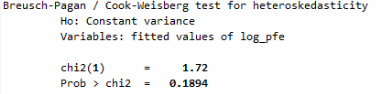
\includegraphics{screenshot021}
	%	\caption{}
	\label{fig:screenshot019}
\end{figure}


Ошибки гомоскедастичны (но на всякий случай будем использовать робастные оценки). В результате, чем чаще посещаются семинары, тем точнее прогнозы, чем выше результаты за 1-ый экзамен, тем точнее прогнозы. 




\subsection{Выводы:}
\begin{itemize}
	\item посещение семинаров не влияет на оценку за экзамен, однако влияет на ожидания;
	\item количество сданных домашних заданий влияет как на оценки, так и на ожидания;
	\item на ожидания влияют количество посещенных семинаров, количество сданных домашних заданий и оценка за 1-ый экзамен;
	\item фактор $expect$ является значимым фактором для прогноза оценки $exam_2$;
	\item студенты ошибаются в среднем в своих прогнозах на 10 баллов; точнее свои оценки предсказывают те, кто сдавал больше домашних заданий и кто лучше написал экзамен.
\end{itemize}






\newpage
\subsection{Программа для STATA:}

\begin{verbatim}

clear
set more off
cd C:\Users\kasyanova\Desktop\stata

log using homeass2_kasianova_shulyak.log, text replace

import excel data_HW_02.xlsx, clear sheet("Sheet1") firstrow

drop if missing(SHW)
drop if missing(Expect)
drop if Expect=="no"
drop if exam1=="n/a"

generate f:f = (man == "")
destring exam1 Expect exam2, replace
recast int NA NHW f exam1 exam2 Expect

generate mean_SHW:mean_SHW = SHW/NHW
replace mean_SHW = 0 if  mean_SHW == .

generate f_mean_SHW:f_mean_SHW = f*mean_SHW

// part I
regress exam2 NA NHW mean_SHW exam1 f f_mean_SHW
regress exam2 NA NHW mean_SHW exam1 f f_mean_SHW Expect
predict res, resid

test NA f f_mean_SHW

regress exam2 NHW mean_SHW exam1 Expect
kdensity  res, normal
swilk res
estat hettest

// part II
regress Expect NA NHW mean_SHW exam1 f f_NA
regress Expect NHW exam1
estat hettest

scatter Expect NHW

regress Expect NA NHW mean_SHW exam1 f f_NA [aweight = NHW], vce(hc3)
estat hettest

test NA mean_SHW f f_NA
test NA f f_NA
test mean_SHW f f_NA

regress Expect NA NHW exam1 [aweight = NHW], vce(hc3)
predict resexp, resid
kdensity  resexp, normal
swilk resexp
estat hettest

// part III
regress exam2 Expect
predict fe, resid
generate afe:afe = abs(fe)
generate pfe = fe/exam2
generate log_pfe: log_pfe = log(abs(pfe))

scatter exam2 pfe
scatter exam2 log_pfe

regress afe NA NHW SHW exam1 f f_mean_SHW
estat hettest
regress afe NA NHW SHW exam1 f f_mean_SHW [aweight = NHW], vce(hc3)
estat hettest

regress log_pfe NA NHW mean_SHW exam1 f
test NA mean_SHW f
regress log_pfe NHW exam1
estat hettest

log close


\end{verbatim}






\end{document}
